\documentclass[12pt, letterpaper]{article}
\usepackage[letterpaper, portrait, margin=1in]{geometry}   %For page Setup
\usepackage[utf8]{inputenc}
\usepackage{amssymb, amsmath}               %For Equations and Formulas
\usepackage{comment}                        %For Commenting
\usepackage{hyperref}                       %For Hyperlinks
\usepackage{listings}                       %For Coding Examples
\usepackage[table]{xcolor}                  %For Coloring Tables
\usepackage{xcolor}                         %For Color Associated with Coding Examples
\usepackage{multicol}                       %For Making Multiple Columns
\usepackage{multirow}                       %Allows for multiple cells in one row in a table
\usepackage{cancel}						%Allow for diagonal strikthroughs
\usepackage{float}						%Keep included images in place
\usepackage{graphicx, epstopdf}                       %Converts eps files to pdf
\usepackage{import}                     % Import Files into document
\usepackage{tikz}                       % Create Diagrams using LaTeX
\usepackage{circuitikz}                 % Create Circuit Diagrams
\usepackage{pdfpages}
\epstopdfsetup{update}

\title{PCB Project Description}
\author{Karl Ventayen}
\date{June 23, 2022}

\usepackage{natbib}
\usepackage{graphicx}

\hypersetup{                                %Setup for Hyperlink Colors
    colorlinks=true,
    linkcolor=blue,                         %For Hyperlinked Text
    filecolor=magenta,                      %For Text that Hyperlinks to other Files
    urlcolor=cyan,                          %For Hyperlinked Printed URLs
}



\begin{document}

\begin{comment}
\begin{titlepage}
    %\titlepage
    \maketitle
\end{titlepage}
\end{comment}

\maketitle

\tableofcontents{}

\section{Introduction}
In the development of hardware today most if not all hardware requires the use of Printed Circuit Boards or PCBs. Compared to other methodologies for assembling circuits such as breadboards and freeform circuit assemblies the usage of PCBs provides solutions that have a better formfactor, mechanical properties, and asthetic.\\
\\
However since the process for producing PCBs is a very involed process this project has been designed to step through how to produce a PCB from Schematic to Assembly to Production.

\section{Project Schematic Diagram}
On the following page the Schematic Diagam for the PCB Project is provided.\\
Note: This design originates from an assignment written by \href{https://www.csuchico.edu/eece/faculty-staff/faculty/meghdad-hajimorad.shtml}{Dr. Meghdad (Amin) Hajimorad}. The assignment name is \href{run:./assets/MiniProject_Description_EECE211Fa2022_UPDATED.pdf}{MiniProject\_Description\_EECE211Fa2022\_UPDATED.pdf}\\
\\
This is an analog multiplier. $<Answer what is an anlog multiplier and how is it implemented.>$
%\includegraphics{./../circuit.pdf}
\includepdf[pages=-]{./assets/circuit.pdf}
%\import{./}{schematic_diagram.tex}

\section{Bill of Materials}
All of these materials are distributed by the CSU Chico IEEE, therefore component prices provided on the table below are according to them.\\
\\
Note:
\begin{enumerate}
    \item All of these components are Through-Hole Components.
    \item Footprint IDs refer to names that are provided in the KiCad 7 Library
\end{enumerate}

\begin{center}
    \begin{tabular}{|c|c|c|c|}
        \hline
        Component & Identification & Footprint & Price\\ 
        \hline
        Resistors & Carbon Film & Resistor\_THT:R\_Axial\_DIN0309\_L9.0mm\_D3.2mm\_P15.24mm\_Horizontal& \\  
        \hline
        Diode & 1N4148 & Diode\_THT:D\_DO-35\_SOD27\_P7.62\_Horizontal & cell9 \\
        \hline
        Pin Headers & Conn\_01x03\_Pin & Connector\_PinHeader\_1x03\_P2.54mm\_Vertical& \\
        \hline
        Operational Amplifier & LF347N & Package\_DIP:DIP-14\_W7.62mm\_Socket & \\
        \hline
        Operational Amplifier & TL084CN & Package\_DIP:DIP-14\_W7.62mm\_Socket & \\
        \hline
    \end{tabular}
\end{center}

\section{Scematic Layout}
For the schematic layout ensure that you have the following parameters included into your diagrams and netlists.

\section{PCB Board Layout}
For the PCB Board Layout ensure that you have the following parameters included in your design.

\section{Production}
The selected group to produce the Boards for this project is OSH Park. Be sure to upload the file with the right parameters addressed to make sure that the board works appropriately.

\section{Assembly}
Collect all of the components and make sure that you collect all of the appropriate components and assemble them in accordance to your design. If you have any descrpancies with understanding your board you can consult your schematic diagram on KiCad.

\section{Testing}
Testing will happen with the use of An Oscilloscope, Waveform Generator, DC Power Supply, and Multimeter.
\end{document}